%Dit is een standalone TeX. Deze wordt gecompiled als main.tex een andere preamble heeft als dit bestand, bijvoorbeeld oneside op titelpagina, twoside in main.tex

\documentclass[10pt,a4paper,oneside]{article}
\usepackage[utf8]{inputenc} %Codering
\usepackage[dutch]{babel} %Taalinstelling
\usepackage{biblatex} %Om een of andere reden wil deze TeX niet compilen zonder deze package, deze is niet nodig
\usepackage{csquotes} %Deze is ook nodig om errors tegen te gaan, hoewel hij zelf niet nodig is
\usepackage[pages=some]{background}

\usepackage{graphicx}
\graphicspath{ {../Images/} }

\usepackage[linktoc=all]{hyperref}
\hypersetup{colorlinks=false} %Links naar websites, bronnen, inhoudsopgave, pagina's etc.

\usepackage[a4paper, margin=2.5cm]{geometry}

\usepackage{titling} %Titels voor op de titelpagina
\def\titel{\textbf{Treasury letter} \\
\vspace*{0.3cm}
{\huge Seafood Connection B.V.}}
\def\ondertitel{}

\def\organisatie{Seafood Connection B.V.}
\def\mailorganisatie{info@seafoodconnection.nl}
\def\telorganisatie{+31 527 687 066}
\def\adres{Het Spijk 12\\
8321 WT, Urk}

\def\auteur{G. Post}
\def\begeleidereen{J.J. Molenaar}
\def\begeleidertwee{L. Brouwer}

\def\datum{07-01-2019}
\def\terugwerkend{01-01-2018}
\def\uittreden{01-01-2022}
\def\versie{1.0}

\def\vertspace{0.5cm}

\title{\titel}
\author{\auteur}
\date{\datum}
%EIND VAN PREAMBLE


\begin{document}
%\backgroundsetup{contents=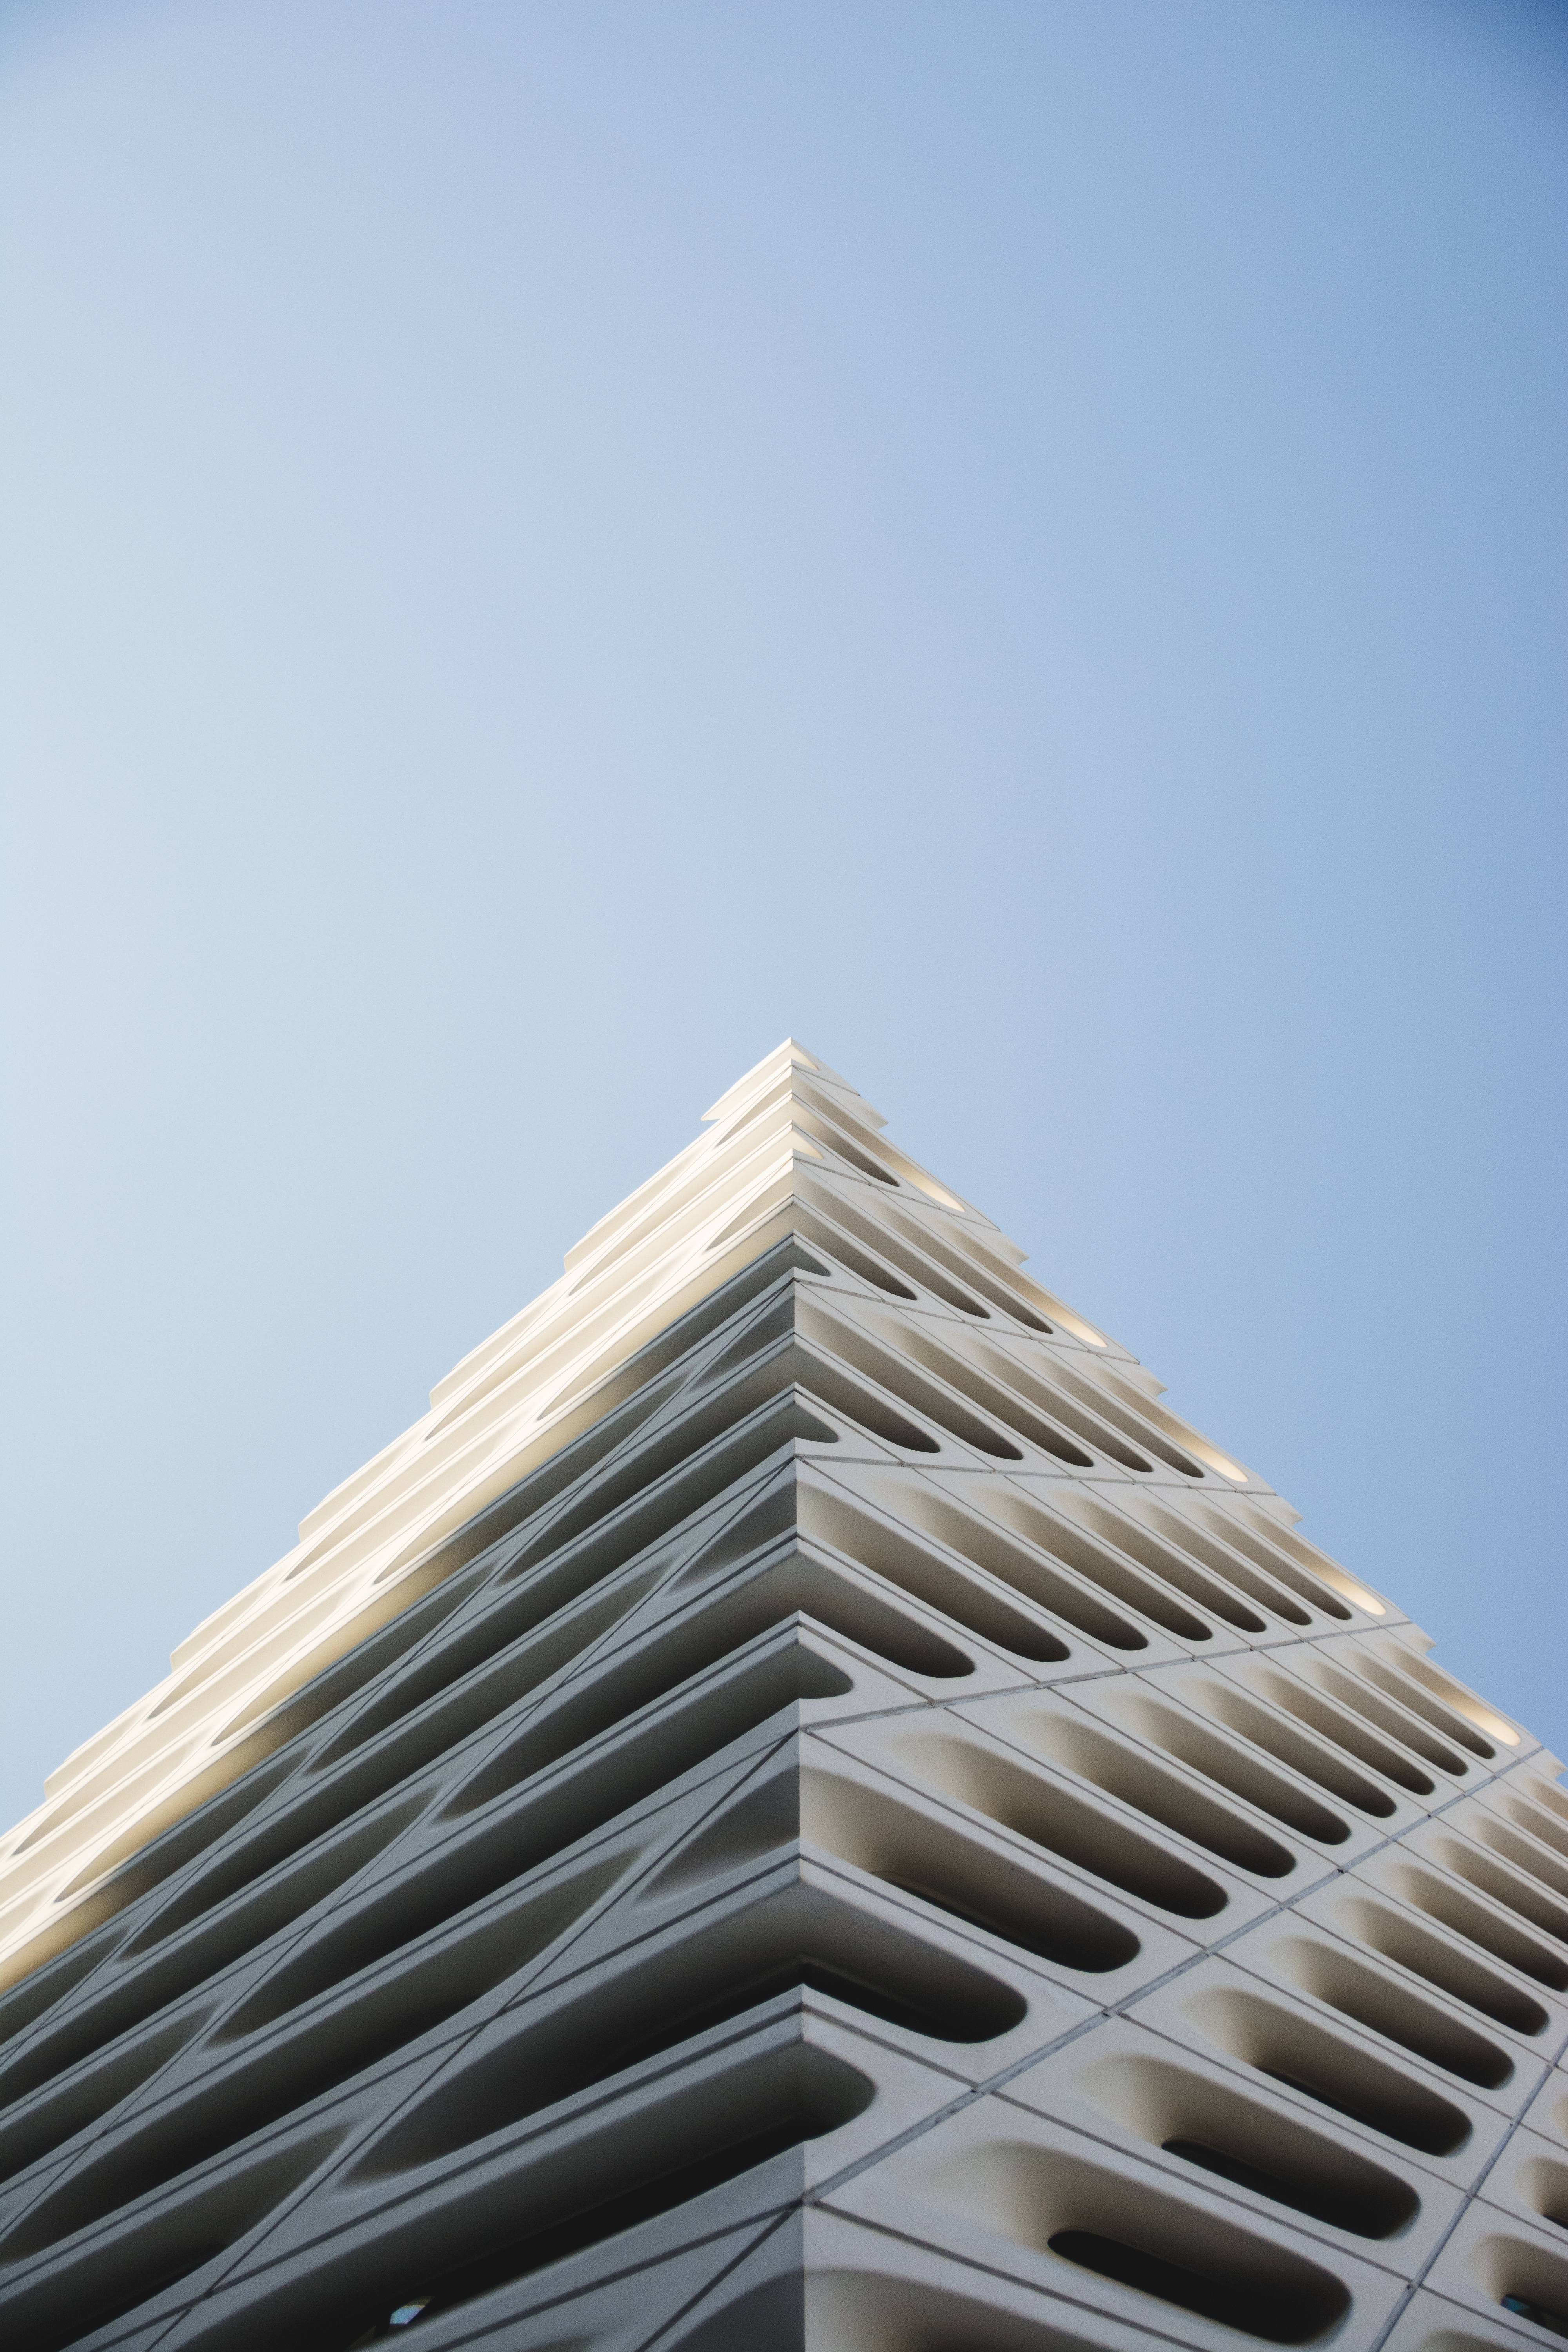
\includegraphics{3},angle=0,scale=0.15,opacity=0.5,vshift=195}
%\backgroundsetup{contents=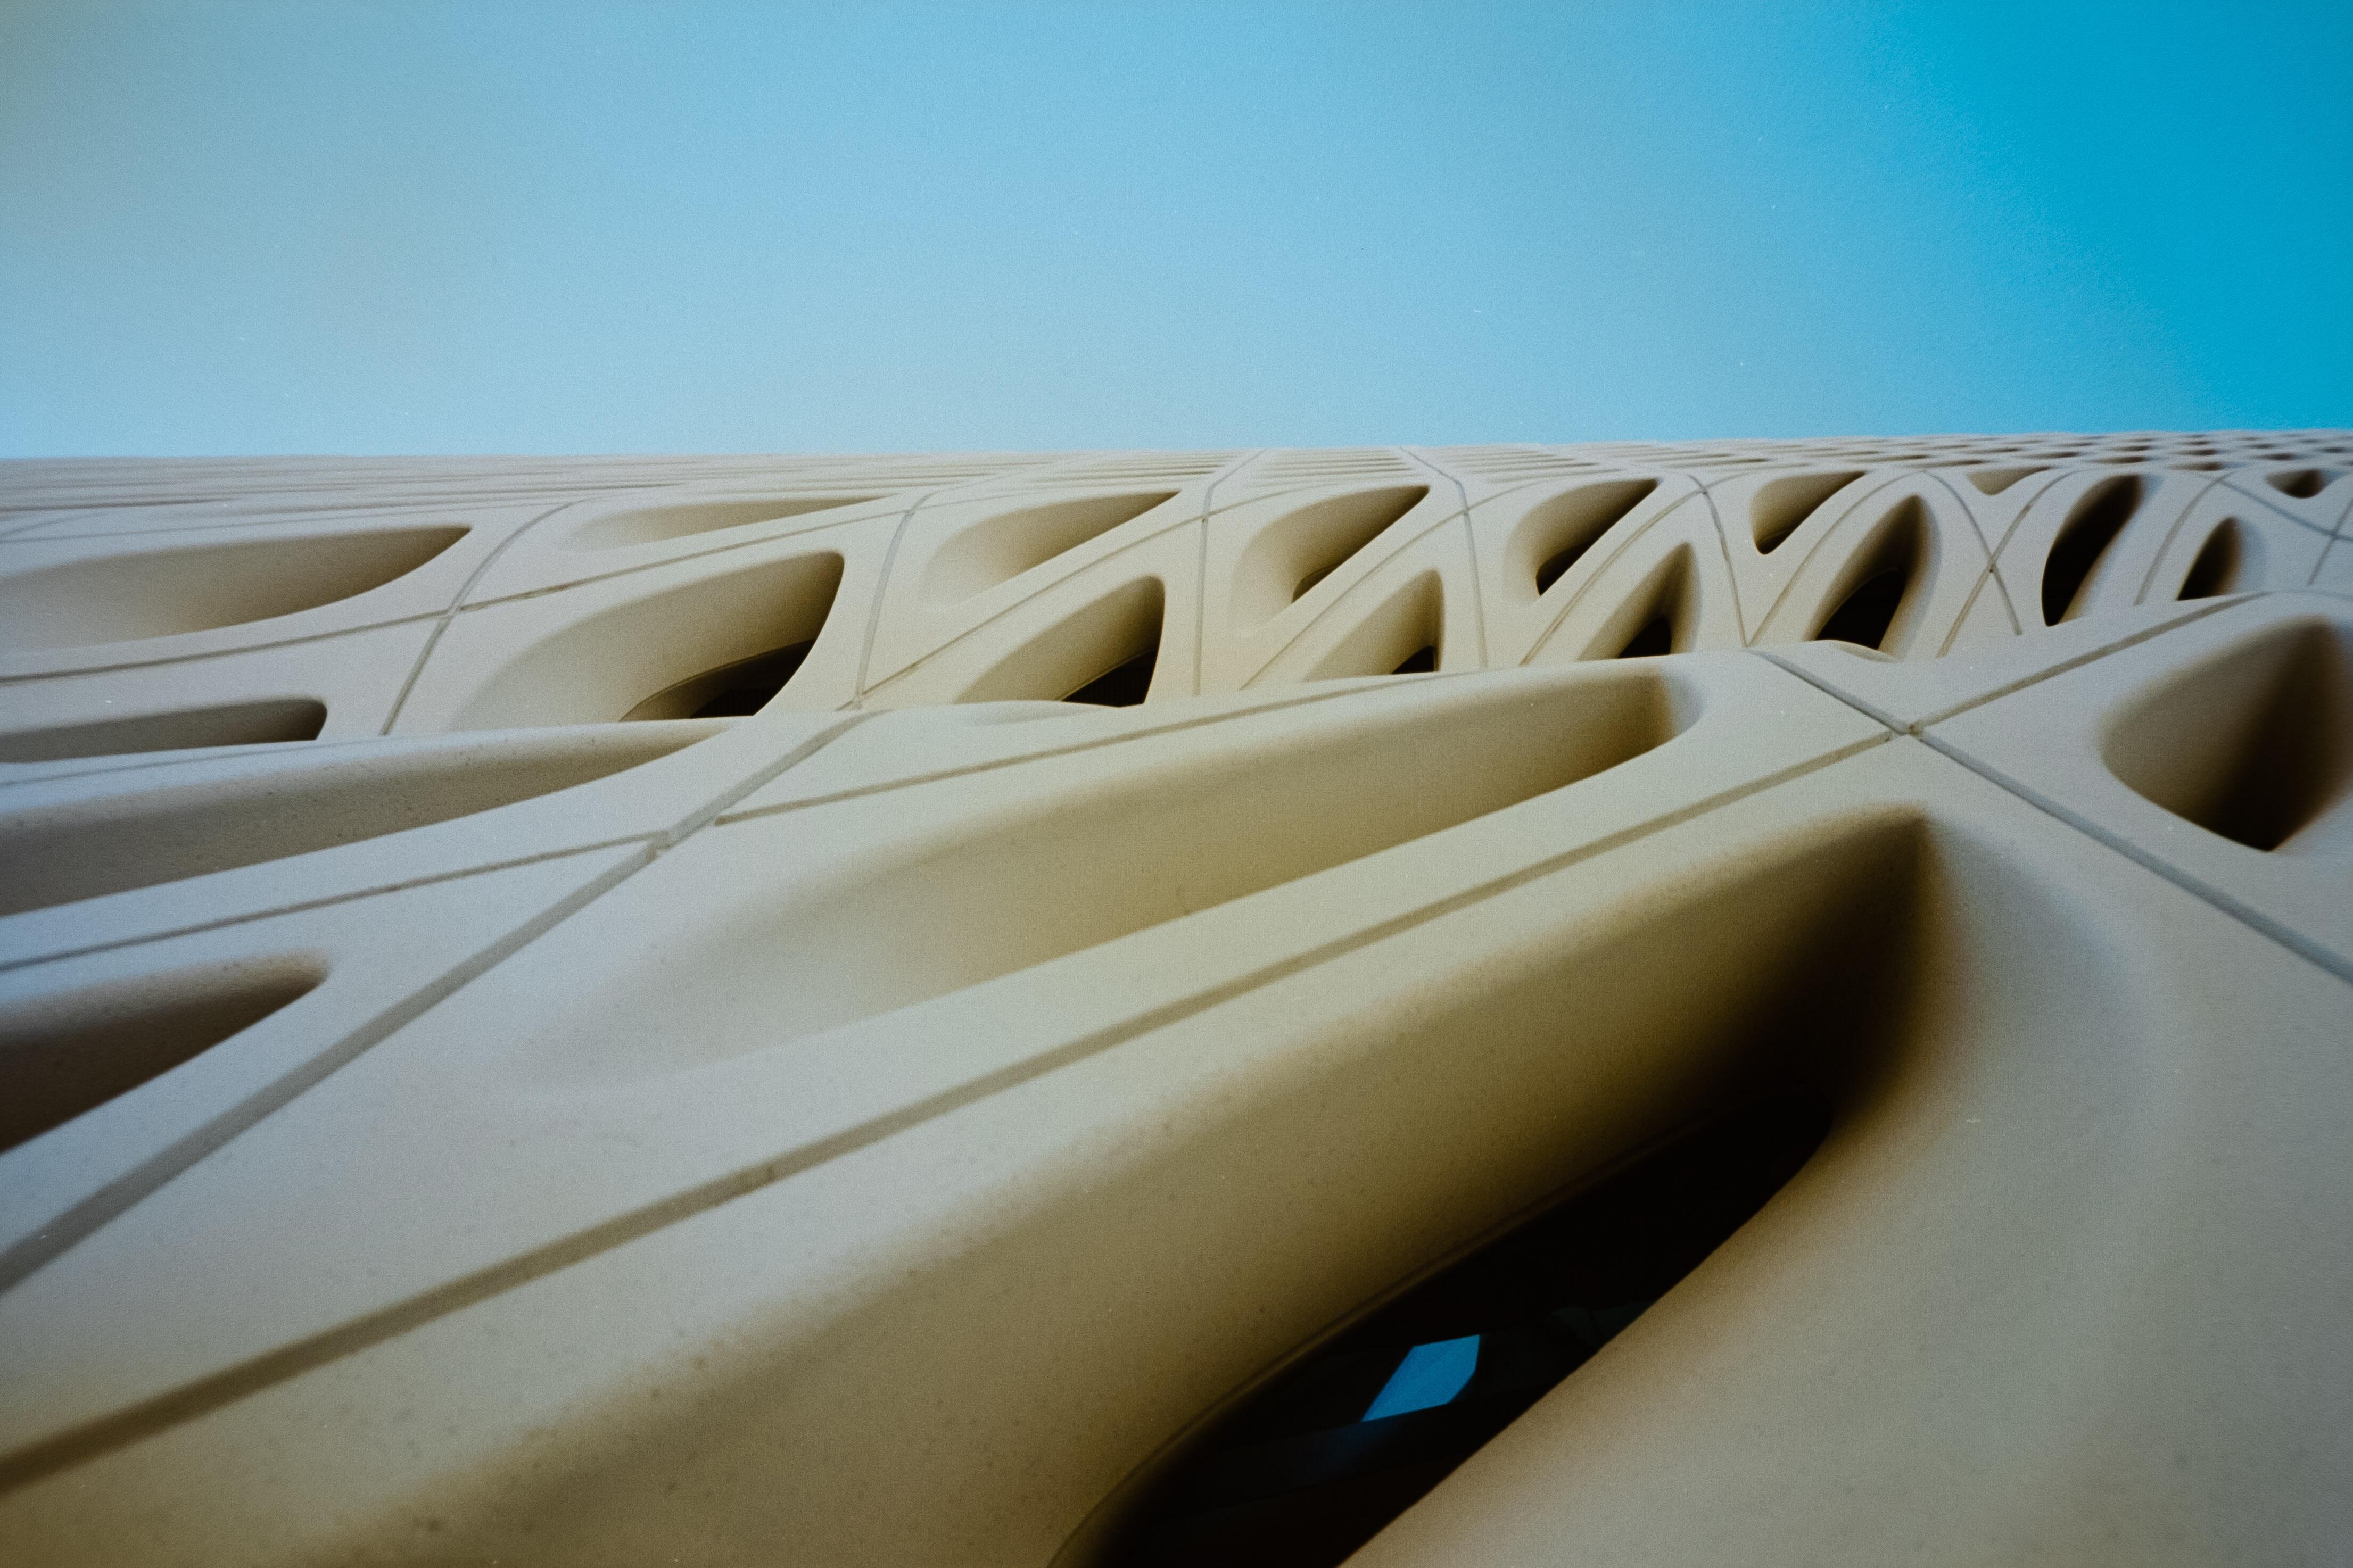
\includegraphics{2},angle=90,scale=0.205,opacity=0.5}
\backgroundsetup{contents=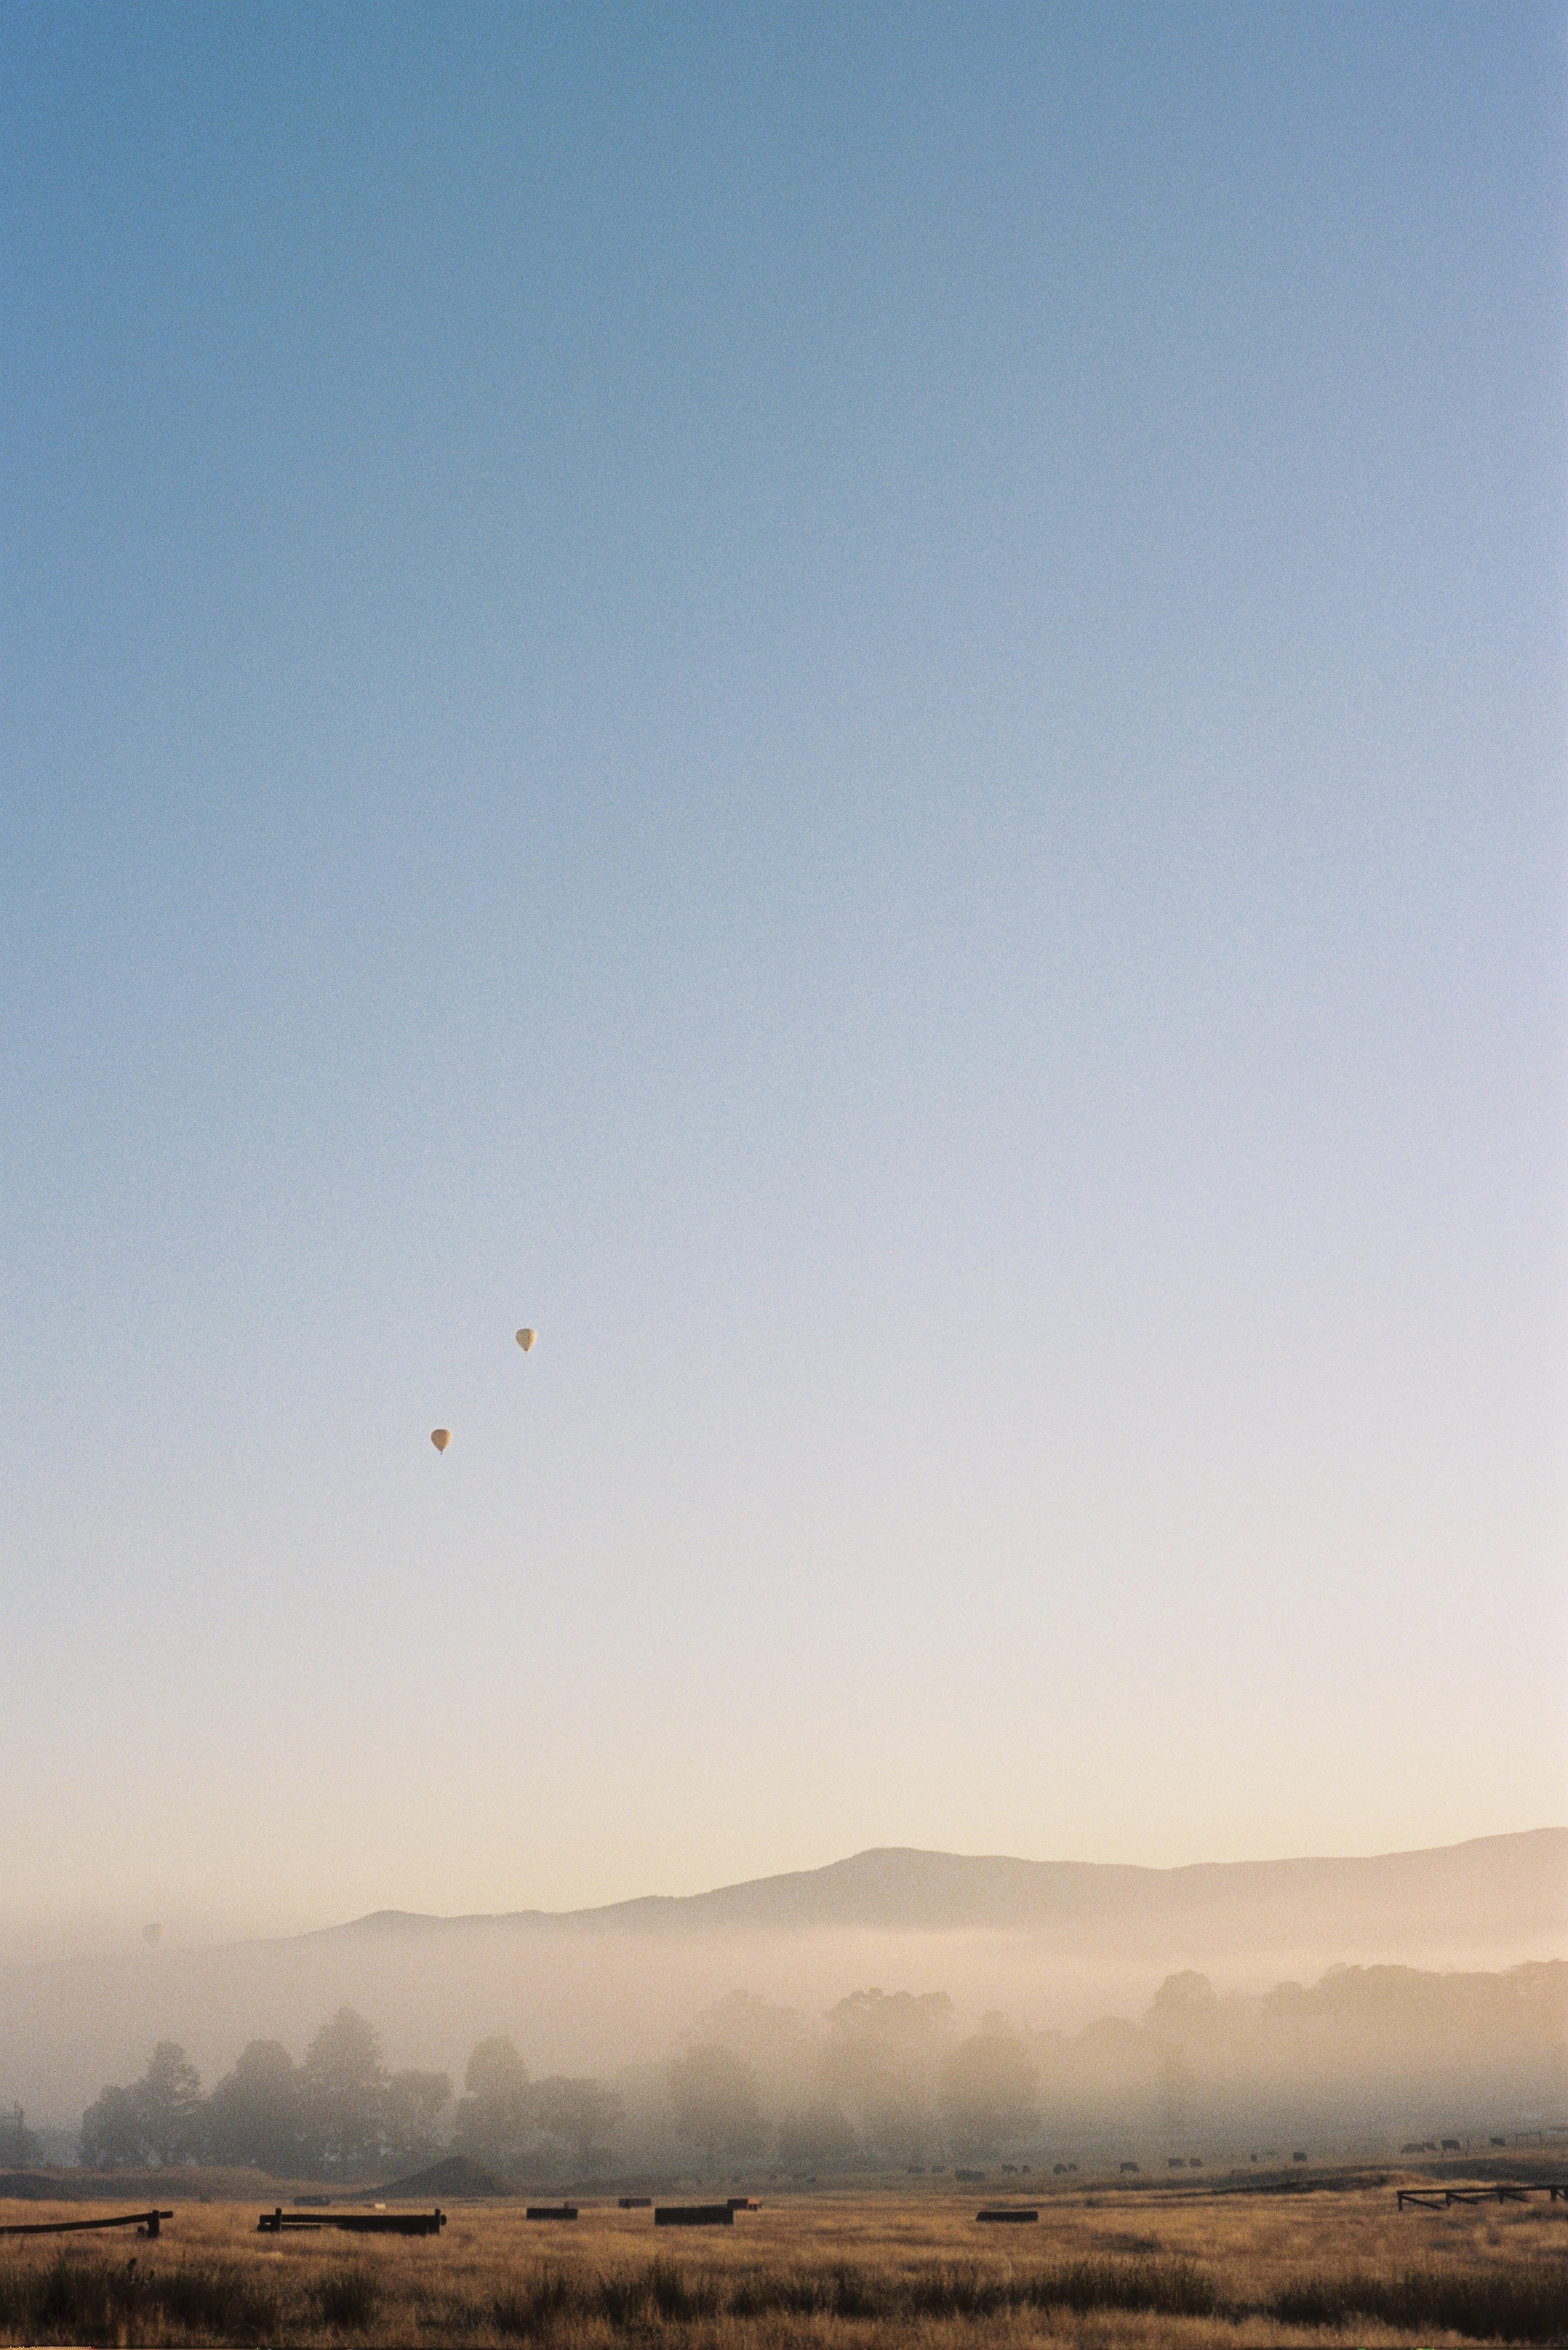
\includegraphics{5},angle=0,scale=0.19,opacity=1,vshift=-400}
\BgThispage
\begin{titlepage}
    \begin{center}
    \vspace*{3cm}
    {\Huge\thetitle}
    
    \vspace*{0.4cm}
    \textnormal{\ondertitel}
    \end{center}
    
    \raggedleft
    \vfill
    \textbf{Authors} \\
    mr. \theauthor \\
    mr. \begeleidertwee \\
    mr. \begeleidereen \\

    \vspace{\vertspace}
    \textbf{Organization} \\
    \organisatie \\
    \mailorganisatie \\
    \telorganisatie \\
    \adres \\
    The Netherlands
    
    \vspace{\vertspace}
    %Versie \versie \\
    Established by the management board on \thedate \\
    Retroactively adapted from \terugwerkend \\
    Valid untill \uittreden
\end{titlepage}

\end{document}